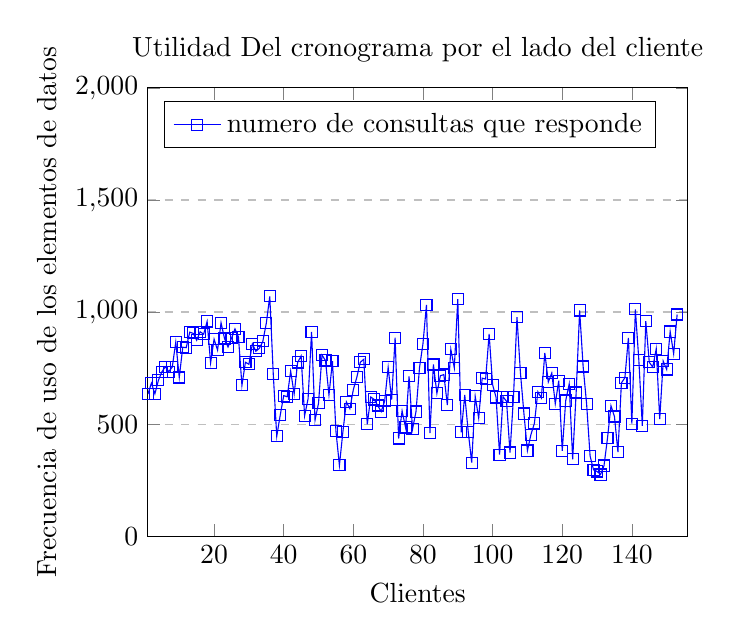
\begin{tikzpicture}
\begin{axis}[
    title={Utilidad Del cronograma por el lado del cliente},
    xlabel={Clientes},
    ylabel={Frecuencia de uso de los elementos de datos},
    xmin=1, xmax=156,
    ymin=0, ymax=2000,
    xtick={},
    ytick={},
    legend pos=north west,
    ymajorgrids=true,
    grid style=dashed,
]

\addplot[
    color=blue,
    mark=square,
    ]
    coordinates {
    %USO EXACTO
    (1,634)
(2,683)
(3,635)
(4,695)
(5,733)
(6,756)
(7,734)
(8,755)
(9,866)
(10,708)
(11,843)
(12,841)
(13,910)
(14,905)
(15,874)
(16,912)
(17,901)
(18,958)
(19,773)
(20,879)
(21,830)
(22,952)
(23,882)
(24,844)
(25,883)
(26,925)
(27,889)
(28,673)
(29,776)
(30,767)
(31,858)
(32,825)
(33,838)
(34,869)
(35,950)
(36,1070)
(37,723)
(38,446)
(39,540)
(40,627)
(41,622)
(42,736)
(43,634)
(44,775)
(45,804)
(46,537)
(47,613)
(48,911)
(49,518)
(50,593)
(51,808)
(52,784)
(53,630)
(54,781)
(55,469)
(56,316)
(57,466)
(58,599)
(59,569)
(60,654)
(61,709)
(62,776)
(63,789)
(64,499)
(65,621)
(66,610)
(67,583)
(68,556)
(69,603)
(70,753)
(71,609)
(72,886)
(73,436)
(74,559)
(75,485)
(76,713)
(77,478)
(78,556)
(79,751)
(80,859)
(81,1032)
(82,460)
(83,766)
(84,637)
(85,716)
(86,721)
(87,585)
(88,834)
(89,751)
(90,1057)
(91,463)
(92,630)
(93,466)
(94,328)
(95,624)
(96,527)
(97,705)
(98,701)
(99,902)
(100,676)
(101,619)
(102,364)
(103,622)
(104,602)
(105,373)
(106,622)
(107,977)
(108,728)
(109,547)
(110,382)
(111,453)
(112,503)
(113,644)
(114,617)
(115,818)
(116,688)
(117,728)
(118,591)
(119,694)
(120,381)
(121,605)
(122,679)
(123,343)
(124,641)
(125,1007)
(126,757)
(127,590)
(128,358)
(129,296)
(130,289)
(131,275)
(132,315)
(133,437)
(134,582)
(135,534)
(136,375)
(137,684)
(138,707)
(139,885)
(140,502)
(141,1012)
(142,786)
(143,492)
(144,959)
(145,776)
(146,754)
(147,836)
(148,522)
(149,781)
(150,744)
(151,913)
(152,814)
(153,989)
    };
    \legend{numero de consultas que responde}

\end{axis}
\end{tikzpicture}

